\clearpage
\section{Simplified Coherent Receiver}

\begin{tcolorbox}	
\begin{tabular}{p{2.75cm} p{0.2cm} p{10.5cm}} 	
\textbf{Student Name}  &:& Romil Patel\\
\textbf{Starting Date} &:& August 16, 2017\\
\textbf{Goal}          &:& Develop a simplified structure (low cost) for a coherent receiver, that can be used in coherent PON, inter-data center connections, or metropolitan networks (optical path lengths should be < 100 km).
\end{tabular}
\end{tcolorbox}

In recent days, homodyne detection has been discussed and investigated a lot due to the advancement in the DSP in the electrical domain. However, a major drawback of homodyne detection is the incoming signal should be separated into inphase and quadrature (I/Q) signals in the optical domain. Therefore, it demands more hardware to accommodate the requirement of the signal separation  in the optical domain. For instance, 4 balanced photodetectors with double hybrid structures and 4-channel ADCs are required.
On the other hand, heterodyne receiver simplifies the detection scheme to some extent with the requirement of having only half of photodetectors and ADC.\\
Such coherent detection scheme constitute the solution for the medium-to-long-reach application; however, the cost of coherent receiver becomes a major obstacle in the case of short-reach links applications like PON, inter-data-center communications, metropolitan network etc. In order to get rid of higher cost and to make the transceiver more efficiently applicable in short-reach links, a new architecture of optical receiver has been proposed which combines the advantages of coherent transmission and cost effectiveness of direct detection. The working principle of the receiver is based on the famous Kramers-Kronig(KK) relationship which facilitates digital post-compensation of linear propagation impairments. The proposed Kramers-Kronig(KK) receiver structure is highly efficient in terms of spectral occupancy and energy consumptions.
\subsection{Minimum Phase Signal}
The communication scheme discussed here relies on the identifying a specific condition that ensures the received signal is minimum phase. This condition facilitates the unique way to extract the phase of the received signal from its intensity. If we denote s(t) as a complex data-carrying signals whose spectrum is contained between -B/2 to B/2, and consider a single sideband signal of the form,
\begin{equation}
h(t)=A+s(t)exp(i\pi Bt)
\end{equation}
Where $A$ is a constant. Here, Nyquist stability criterion can be used to ensure that $s(t)$ is a minimum phase signal. The condition of minimum phase signal is satisfied when $|A|>|s(t)|$ by guaranteeing Nyquist stability of the received signal.
When $h(t)$ is a minimum-phase signal, its phase $\phi(t)$ and absolute value $|h(t)|$ are uniquely related by Hilbert transform:
\begin{equation}
	\phi(t)=\frac{1}{\pi}  p.v. \int_{-\infty}^{\infty} dt' \frac{log[|h(t')|]}{t-t'}
	\label{Eq:5.15}
\end{equation}
where \textit{p.v.} stands for \textit{principal value}. The relationship depicted in Equation \ref{Eq:5.15} can also be conveniently implemented in frequency domain as,
\begin{equation}
\tilde{\phi}(\omega)=i sign(\omega) \mathcal{F} \{log[|h(t)|]\}
\label{Eq:5.16}
\end{equation}
where $sign(\omega)$ is the sign function which is equal to 1 when $\omega>0$, to 0 when $\omega=0$ and to -1 when $\omega<0$. Symbol $\mathcal{F}$ denotes the Fourier transform.
\begin{figure}[h]
	\centering
	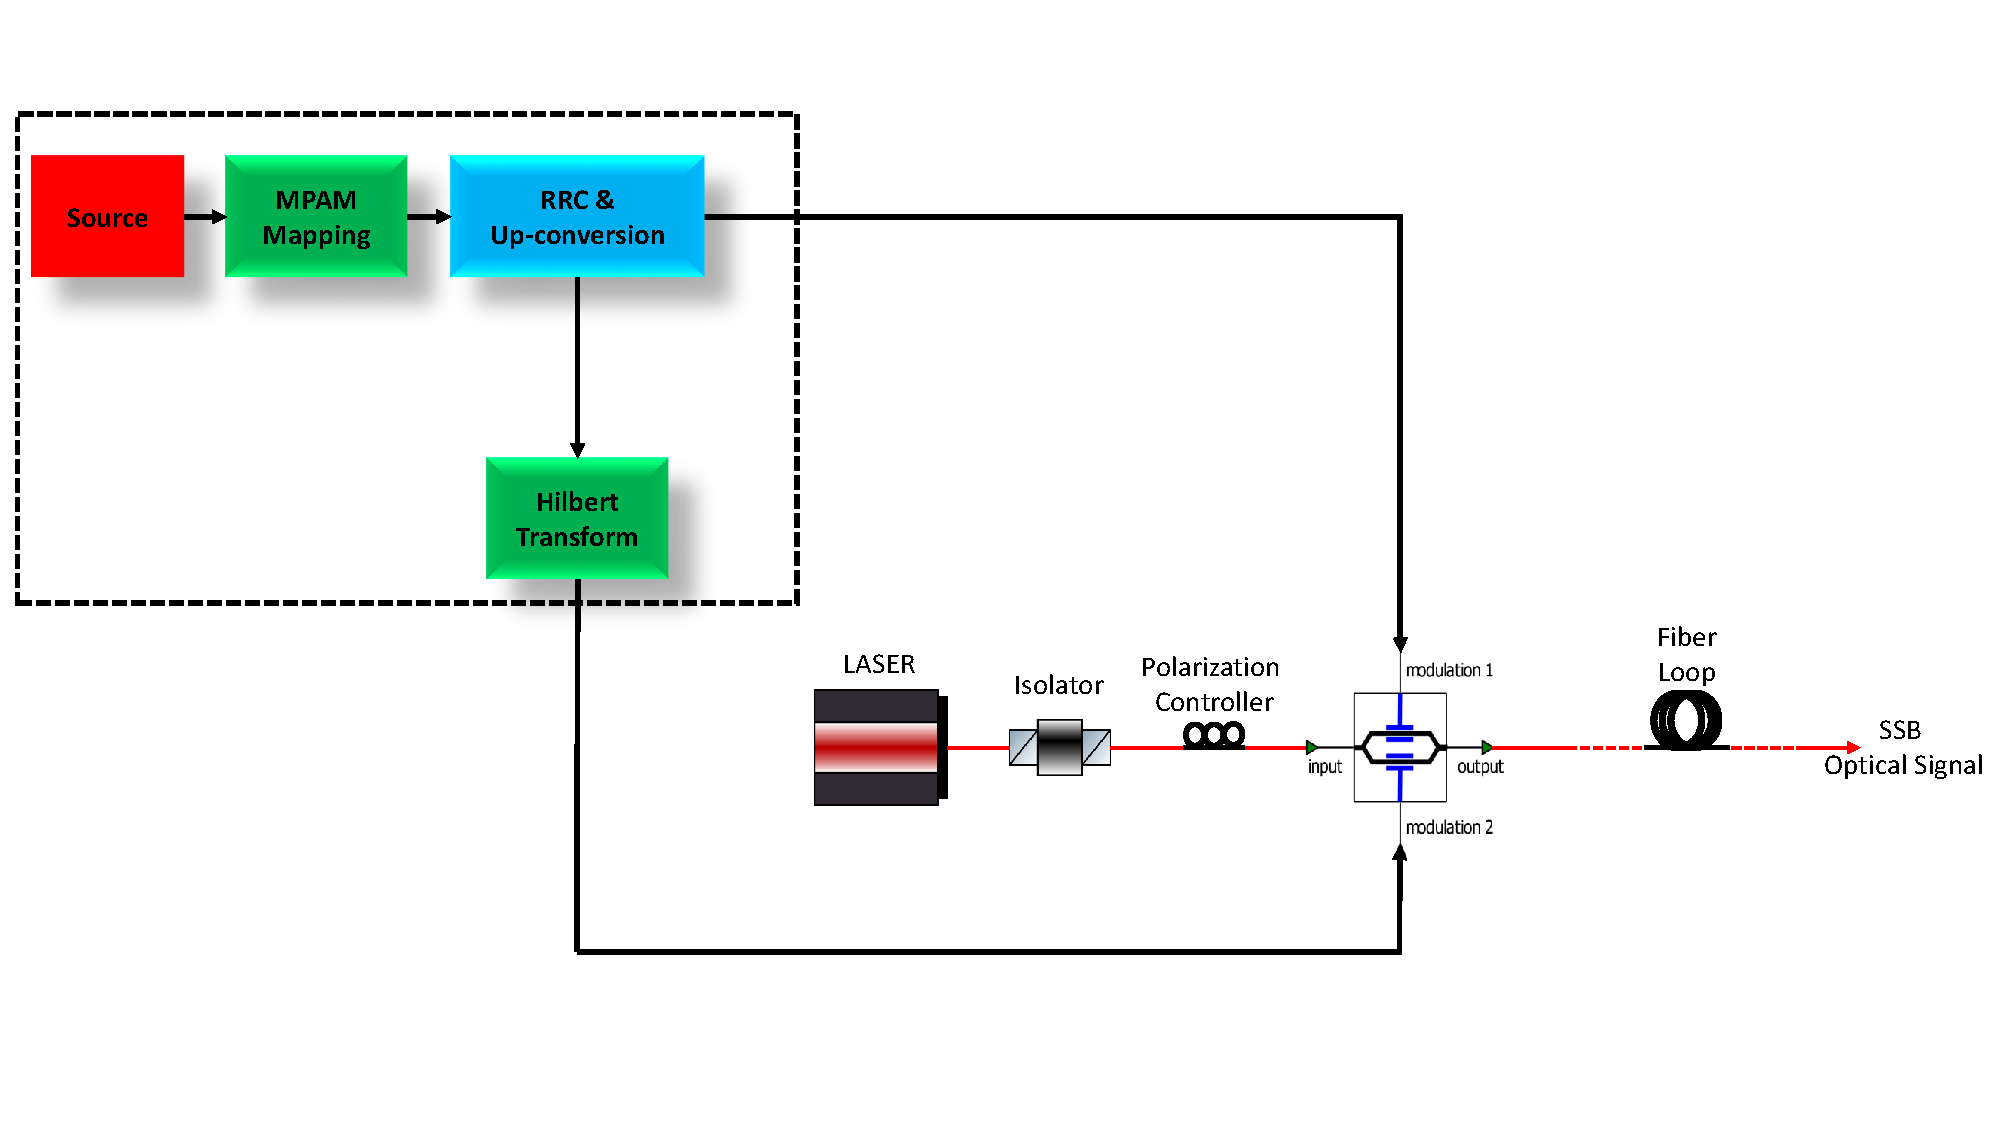
\includegraphics[width=1.0\textwidth, height=7cm]{./sdf/simplified_coherent_receiver/figures/Single_Polarization_Tx.pdf}
	\caption{Transmitter}\label{Transmitter}
\end{figure}

\subsection{KK Scheme}
If we consider the complex envelope of the incoming electric field by $E_s(t)$ confined within the optical bandwidth denoted by B. The LO assumed to be a continuous wave (CW) signal whose amplitude is $E_0$ whose frequency coincides with the left edge of the information-carrying signal spectrum. Here, we assumed that $E_0$ is real-valued and positive, which is equivalent to referring all phase value to that of LO.\\
The complex envelope of the field striking upon the photo-diode can be given as,
\begin{equation}
E(t)=E_s(t)+E_0 exp(i\pi Bt)
\end{equation}
The photo current $I$ produced by the photo-diode is proportional to the field intensity $I=|E(t)|^2$, here proportionality constant considered as 1 for the sake of simplicity. If $E_0$ is large enough to ensure that the signal $E(t)exp(i\pi Bt)=E_0+E_s(t)exp(-i\pi Bt)$ is minimum phase. Equations \ref{Eq:5.15} and \ref{Eq:5.16} can be used to reconstruct the signal $E_s(t)$ as follows:
\begin{equation}
E_s(t)=\{\sqrt{I(t)} exp[i\phi_E(t)]-E_0\} exp(i\pi Bt)
\end{equation}
\begin{equation}
\phi_E(t)=\dfrac{1}{2\pi} p.v. \int_{-\infty}^{\infty} dt' \frac{log[|I(t')|]}{t-t'}
\label{Eq:5.19}
\end{equation}
Here, the average value of the phase returned by Equation \ref{Eq:5.19} is zero, which implies the need for an additional phase-recovery procedure. 
\begin{figure}[h]
	\centering
	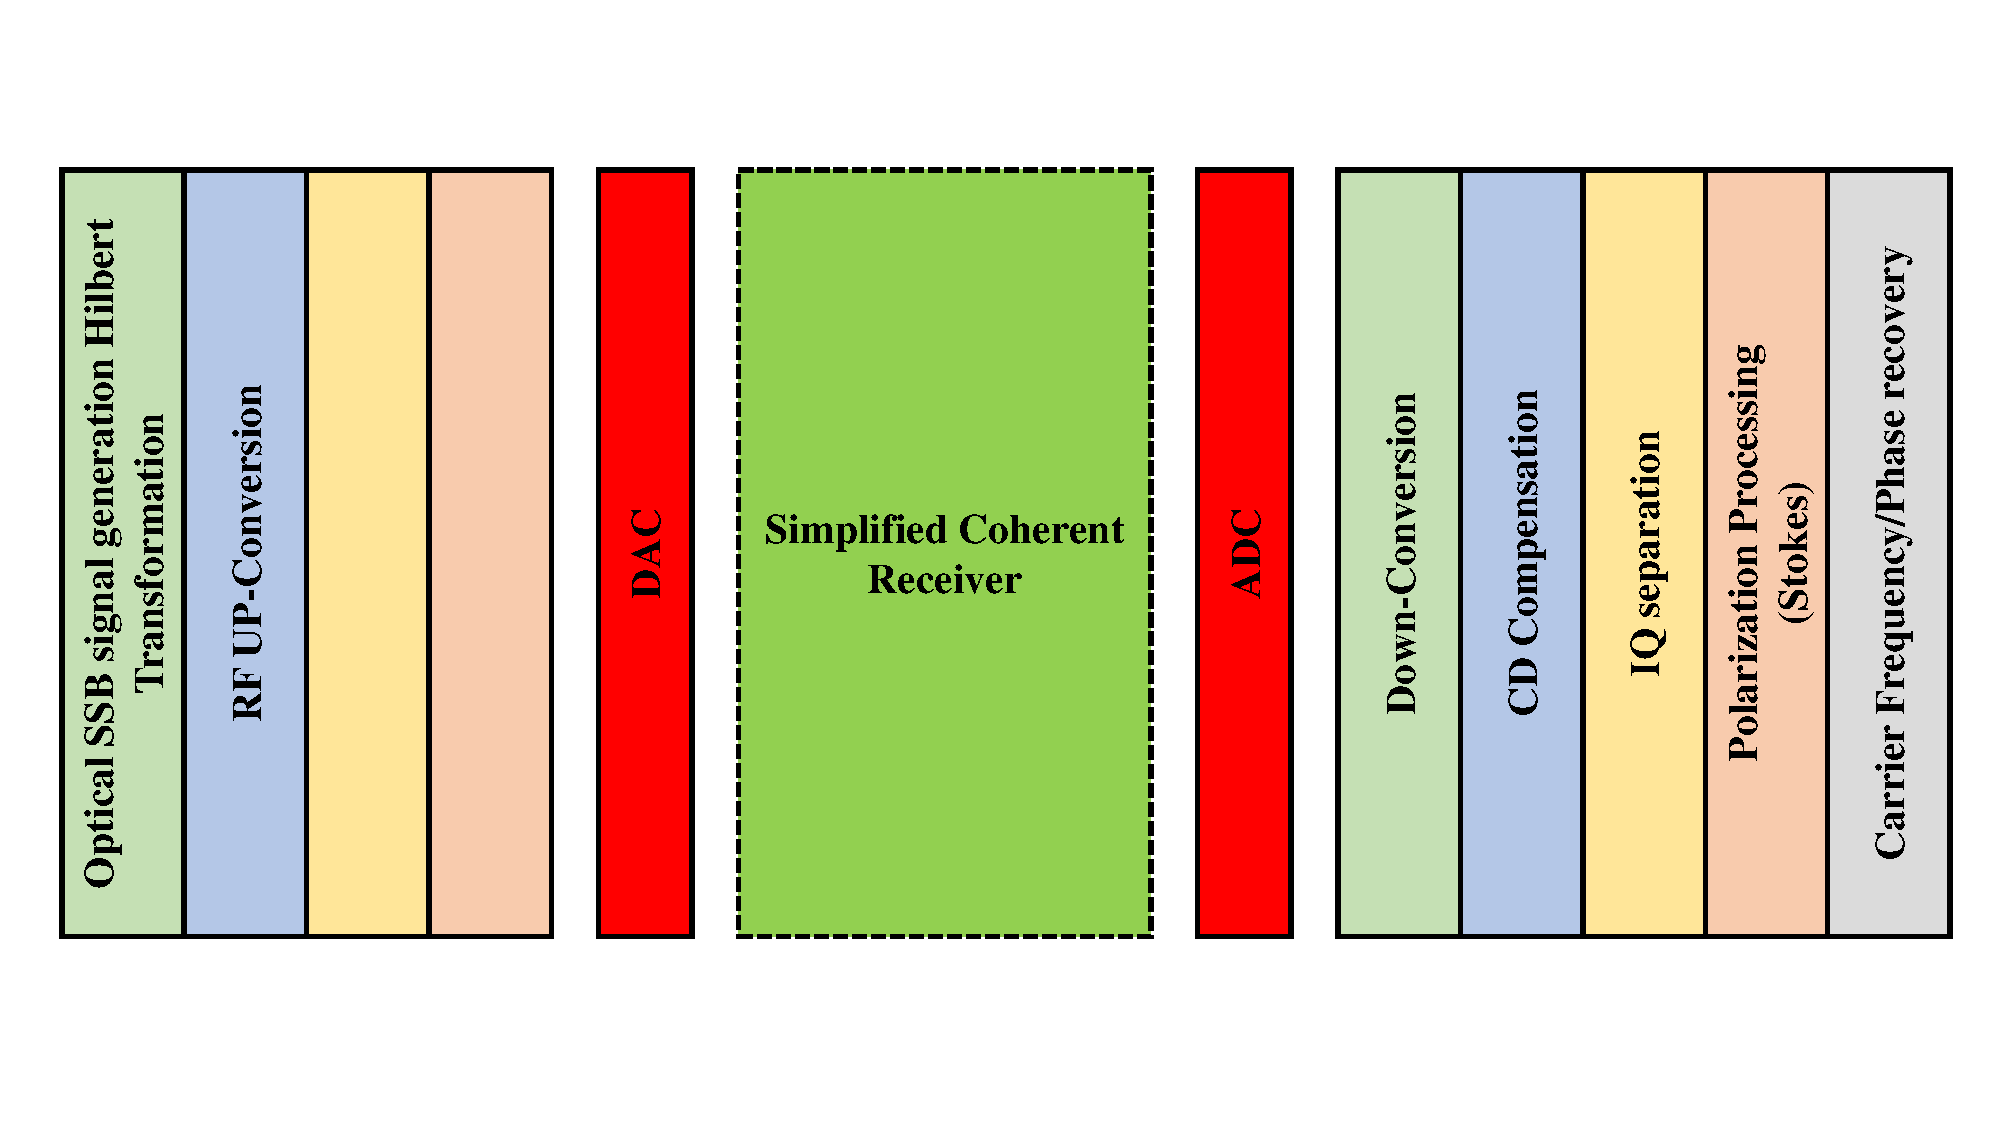
\includegraphics[width=1.0\textwidth, height=8cm]{./sdf/simplified_coherent_receiver/figures/detailed_subsystem.pdf}
	\caption{Tx/Rx DSP main subsystem}\label{DSP_main_subsystem}
\end{figure}

\subsection{Tx side}
Single polarization 16QAM signals (1.25 Gbaud) to be generated at the Tx through an IQ modulator (Figure \ref{DSP_main_subsystem}). The IQ modulated signal is then applied to the Hilbert transformer which generates the imaginary part for our analytical signal. In analytical signal, real and imaginary parts are related to each other by Hilbert transform and it has no negative frequency contents. Such analytical signal can be used for generating bandwidth efficient single sideband (SSB) signal.

\subsubsection{Analytical Signal}
In mathematics and signal processing, an analytic signal is a complex-valued function that has no negative frequency components.The real and imaginary parts of an analytic signal are real-valued functions related to each other by the Hilbert transform.
\begin{equation}
s_a(t)=s(t)+j\hat{s}(t)
\label{Analytical signal}
\end{equation}
where, $s_a(t)$ is an analytical signal and $\hat{s}(t)$ is the Hilbert transform of the signal ${s}(t)$. Such analytical signal can be used to generate SSB signal. In this section, we´ll discuss the brief idea of generating SSB signal using Hilbert transform method. To understand this, we may express signal $s(t)$ as a summation of the two complex-valued functions.
\begin{equation}
s(t)=\dfrac{1}{2}[s(t)+j\hat{s}(t)]+\dfrac{1}{2}[s(t)-j\hat{s}(t)]
\label{}
\end{equation}
where, the term $\dfrac{1}{2}[s(t)+j\hat{s}(t)]$ is the analytical representation of the signal $s(t)$ (from Equation \ref{Analytical signal}). Another term represents the complex conjugate $\dfrac{1}{2}[s(t)-j\hat{s}(t)]$ of this analytical signal. Such representation of the signal ${s_a}(t)$ and ${s_a^*}(t)$ divide the signal into non-negative frequency component and non-positive frequency component respectively. Alternatively, we can write it as,
\begin{equation}
	\dfrac{1}{2}{S_a}(f) = \begin{cases}
		S(f) &\text{for $f>0$}\\
		0    &\text{for $f<0$}\\
	\end{cases}
\end{equation}
where ${S_a}(f)$ and ${S}(f)$ are the Fourier transform of ${t_a}(t)$ and ${s}(t)$ respectively. The frequency translated version of ${S_a}(f-f_0)$ contains only one side (positive) of ${S}(f)$ and hence it is called single sideband signal ${s_ssb}(t)$,
\begin{equation}
{F}^{-1}\{S_a(f-f_0)\}={s_a}(t) e^{j2\pi f_0 t}={s_{ssb}}(t)+j{\hat{s}_{ssb}(t)}
\end{equation}
Therefore, from the Euler's formula,
\begin{equation}
\begin{split}
{s}_{ssb}(t)&=Re\{s_a(t)  e^{j2\pi f_0 t}\}\\
&=Re\{[s(t)+j\hat{s}(t)] [cos(2\pi f_0t)+jsin(2\pi f_0t)]\}\\
&=s(t)cos(2\pi f_0t)-\hat{s}(t)sin(2\pi f_0t)
\end{split}
\label{USB_SSB}
\end{equation}
This Equation \ref{USB_SSB} displays the mathematical modeling of the upper sideband SSB signal. Similarly, we can generate lower sideband SSB signal by,
\begin{equation}
{s}_{ssb}(t)=s(t)cos(2\pi f_0t)+\hat{s}(t)sin(2\pi f_0t)
\label{LSB_SSB}
\end{equation}



\subsubsection{SSB Signal generation using Hilbert transformation}
This section describes the SSB signal generation using Hilbert transformation method (Phase Shift Method). Consider a message signal $m(t)$ with its frequency domain spectrum $M(F)$ as shown in Figure\ref{Original_baseband_signal}. From the Figure \ref{Original_baseband_signal}, we can see that both the side are scaled by factor '1' which means it represents the original signal.
\begin{figure}[h]
	\centering
	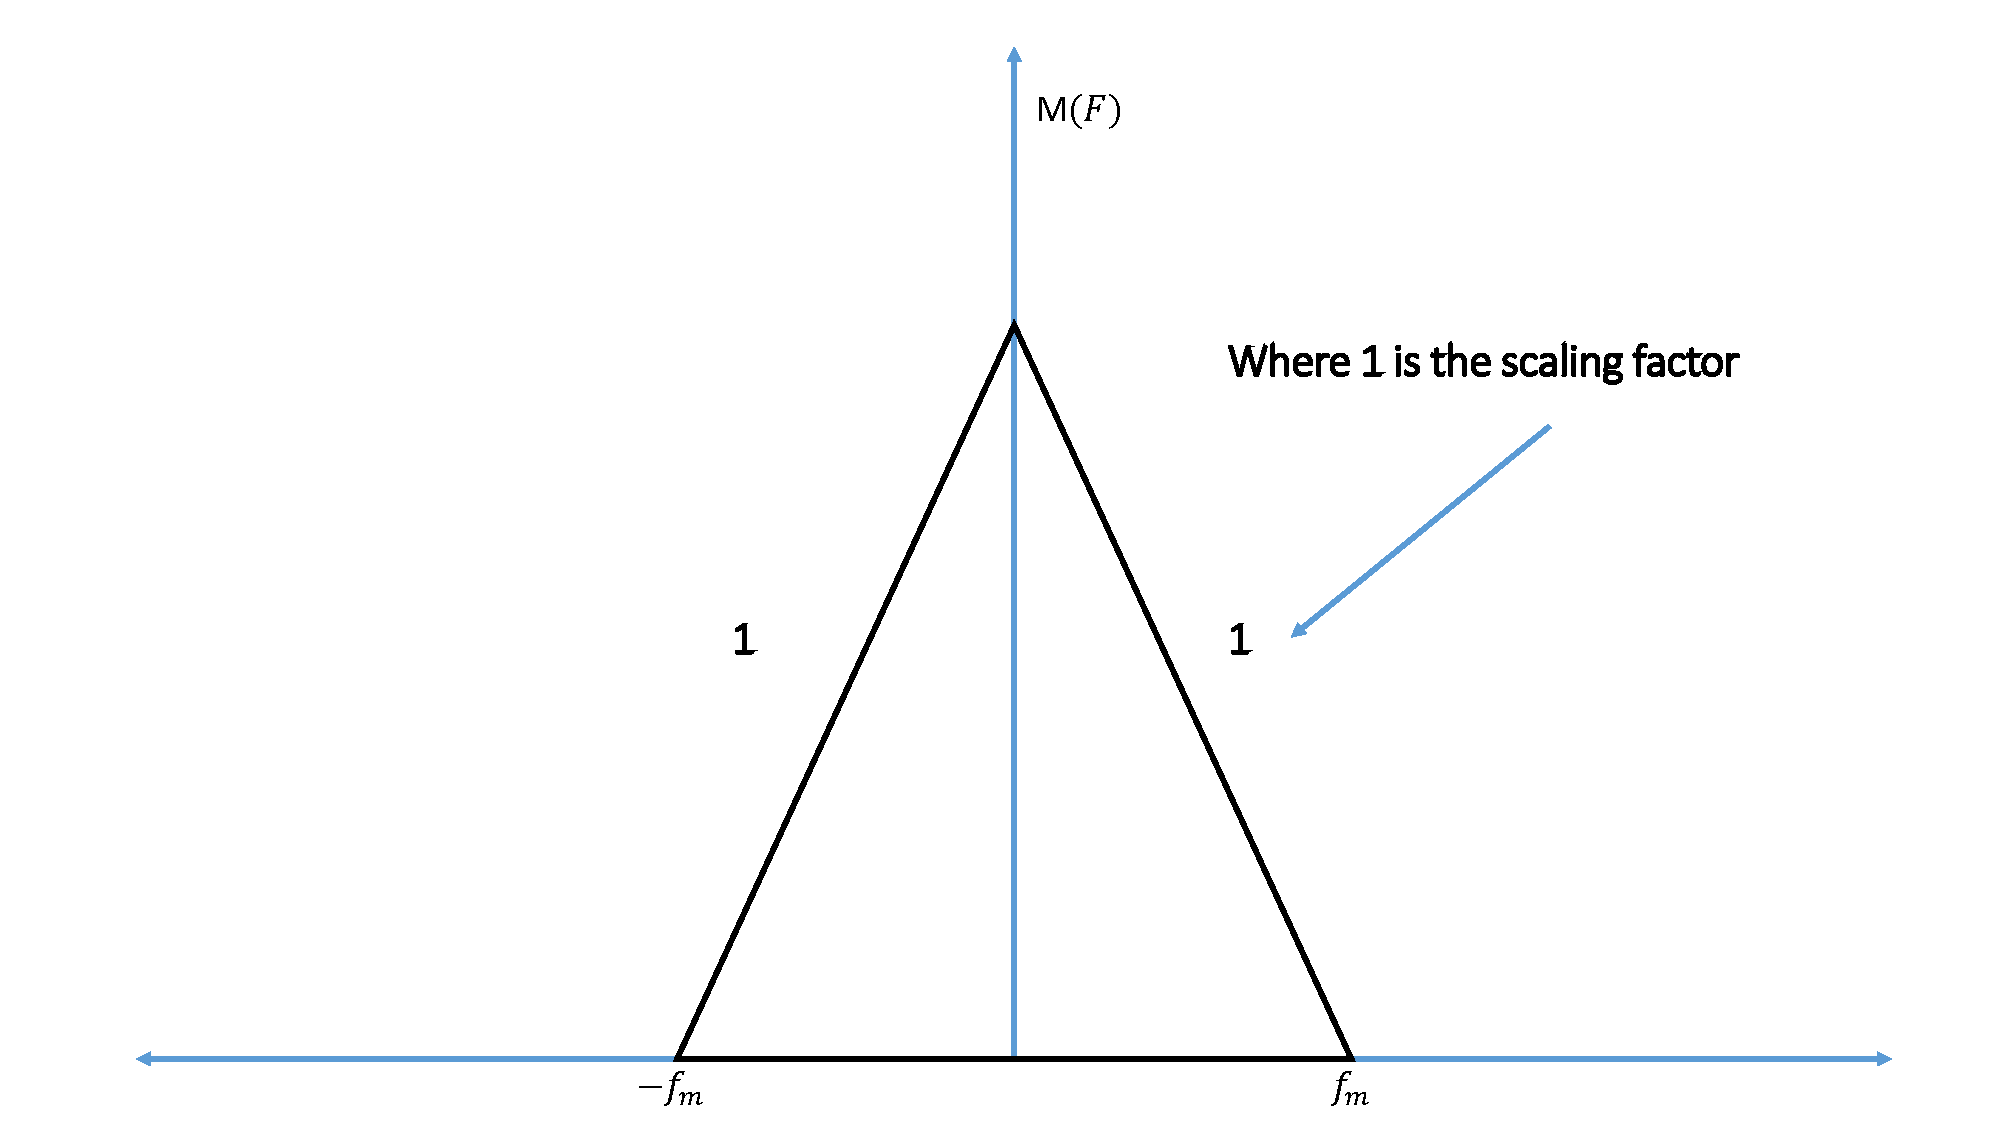
\includegraphics[width=1.0\textwidth, height=8cm]{./sdf/simplified_coherent_receiver/figures/SSB1.pdf}
	\caption{Original baseband signal}\label{Original_baseband_signal}
\end{figure}\\ 	
Now let's consider the modulated signal $x(t)$ given as,
\begin{equation}
x(t)=m(t) cos(2\pi f_c t)
\label{Eq:5.20}
\end{equation}
Frequency domain representation of the equation \ref{Eq:5.20} can be given as,
\begin{equation}
X(F)=\frac{1}{2}M(f-f_c)+\frac{1}{2}M(f+f_c)
\label{Eq:5.21}
\end{equation}
Here in equation \ref{Eq:5.21}, we can observe that each side band are scaled by $\dfrac{1}{2}$ on the frequency spectrum. Figure displays the frequency domain representation of the modulated signal $X(F)$.
\begin{figure}[h]
	\centering
	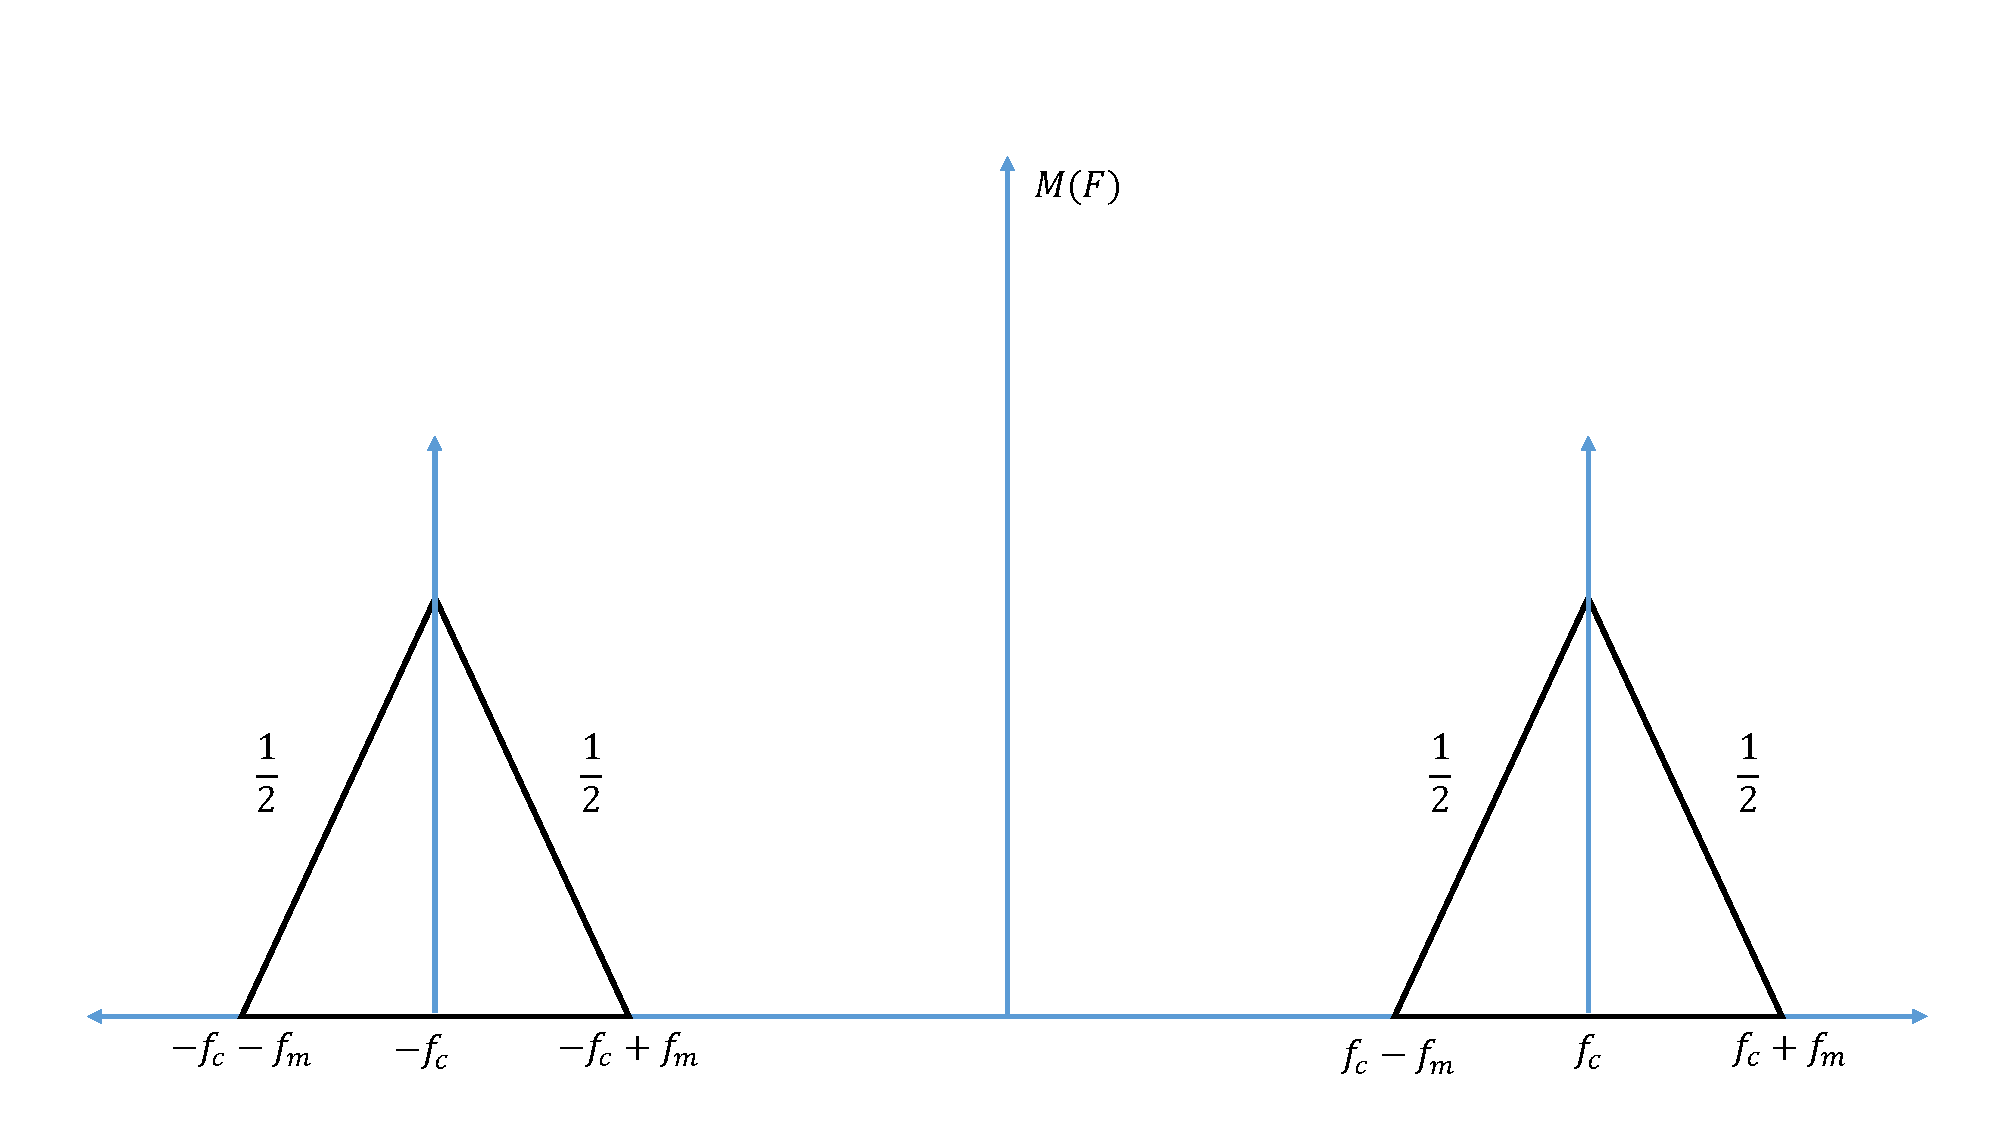
\includegraphics[width=1.0\textwidth, height=8cm]{./sdf/simplified_coherent_receiver/figures/SSB2.pdf}
	\caption{Original modulated signal}\label{Original_modulated_signal}
\end{figure}\\ 
Next, we will discuss something more interesting which is called as Hilbert transform of the original message signal $m(t)$. As we discussed earlier, in the frequency domain, the Hilbert transformed signal $\hat{M}(f)$ can be achieved by multiplying the Fourier transformed signal $M(F)$ with $[-j sgn(F)]$.
\begin{figure}[h]
	\centering
	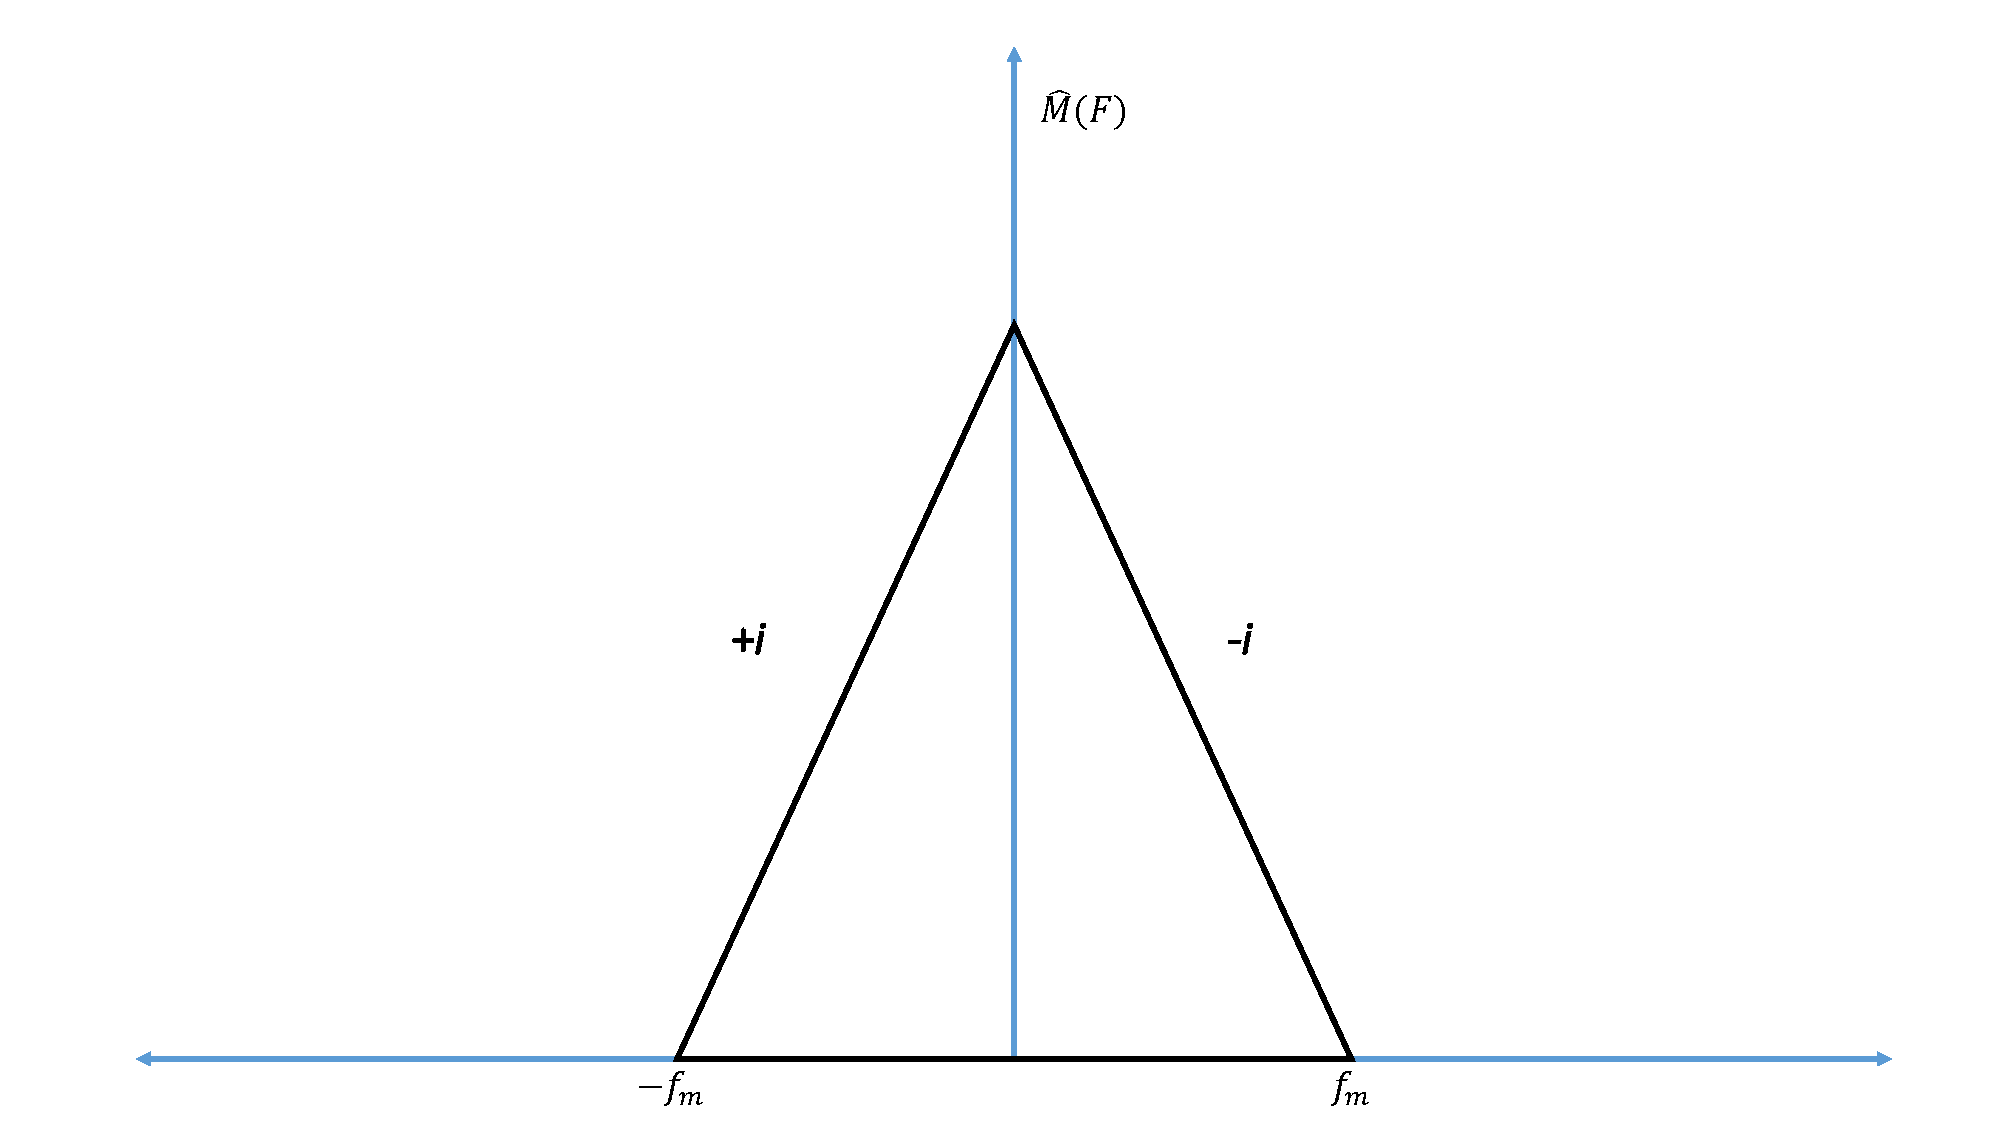
\includegraphics[width=1.0\textwidth, height=8cm]{./sdf/simplified_coherent_receiver/figures/SSB3.pdf}
	\caption{Hilbert transformed modulated signal}\label{Hilbert_Transformed_signal}
\end{figure}
Suppose we modulate the Hilbert transformed message signal $\hat{m}(t)$  with the $sin(2\pi f_c t)$ (quadrature phase carrier), then we get the following results:

\begin{equation}
\begin{split}
{\hat{m}(t)} sin(2\pi f_c t)&={\hat{m}(t)}\frac{e^{j2\pi f_c t} - e^{-j2\pi f_c t} }{2}\\
&={\hat{m}(t)}\frac{e^{j2\pi f_c t}}{2} - {\hat{m}(t)}\frac{e^{-j2\pi f_c t}}{2}\\
&={\frac{\hat{M}(f-f_c)}{2j}}-{\frac{\hat{M}(f+f_c)}{2j}}\\
&={\frac{-j}{2}\hat{M}(f-f_c)}+{\frac{-j}{2}\hat{M}(f+f_c)}\\
\end{split}
\label{5.22}
\end{equation}
The detailed explanation of the equation \ref{Eq:5.22} has been described in the Figure \ref{Hilbert_Transformed_modulated_signal} and \ref{Hilbert_Final}. Figure \ref{Hilbert_Transformed_modulated_signal} displays the spectrum of the $\hat{M}(f+f_c)$ and $\hat{M}(f-f_c)$ for the positive and negative frequencies respectively. The final equation resolution of equation displays that both positive and negative side of the spectrum multiplied with $\frac{j}{2}$ and $\frac{-j}{2}$ respectively. Finally the spectrum of the signal ${\hat{m}(t)} sin(2\pi f_c t)$ can be given as Figure \ref{Hilbert_Final}.
\begin{figure}[h]
	\centering
	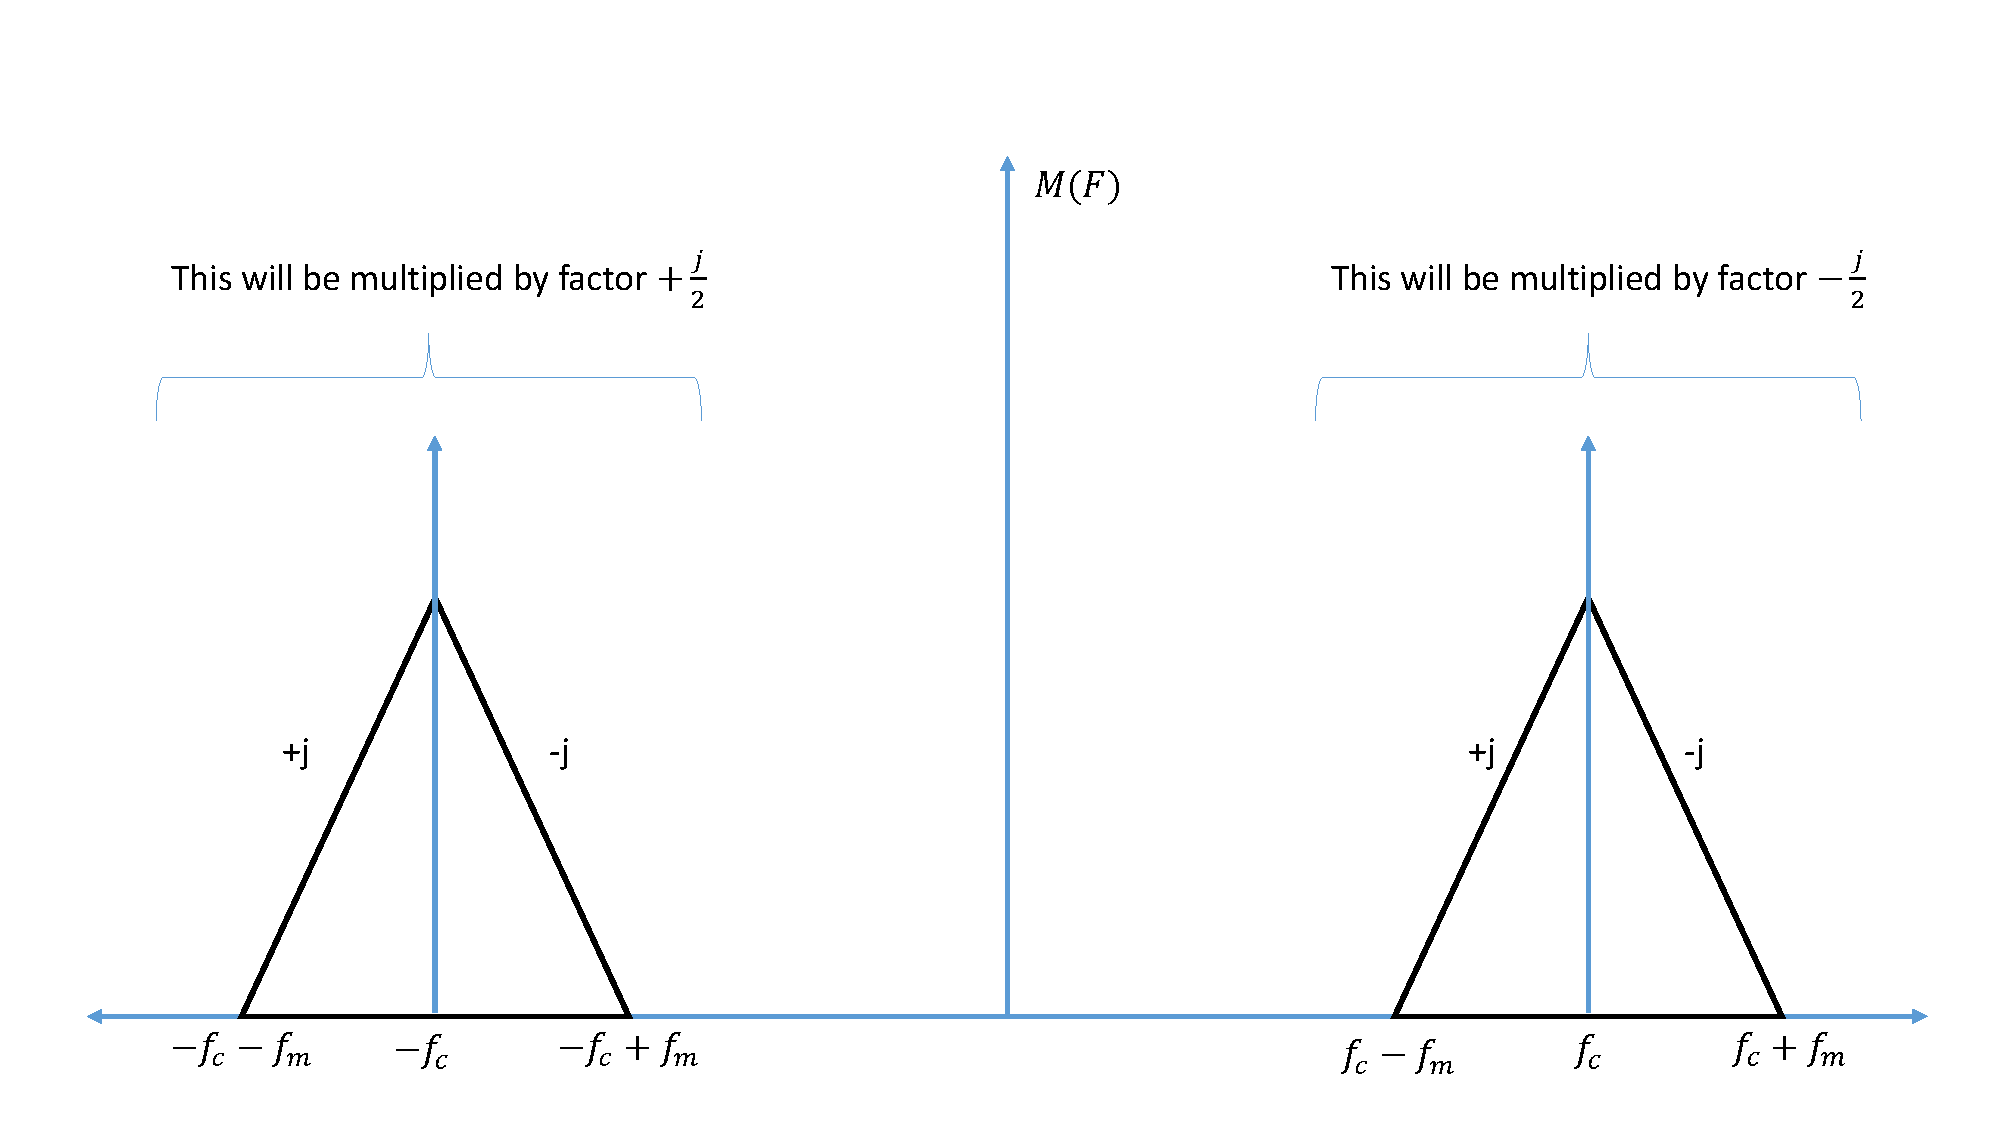
\includegraphics[width=1.0\textwidth, height=8cm]{./sdf/simplified_coherent_receiver/figures/SSB4.pdf}
	\caption{Hilbert transformed modulated signal}\label{Hilbert_Transformed_modulated_signal}
\end{figure}

\begin{figure}[h]
	\centering
	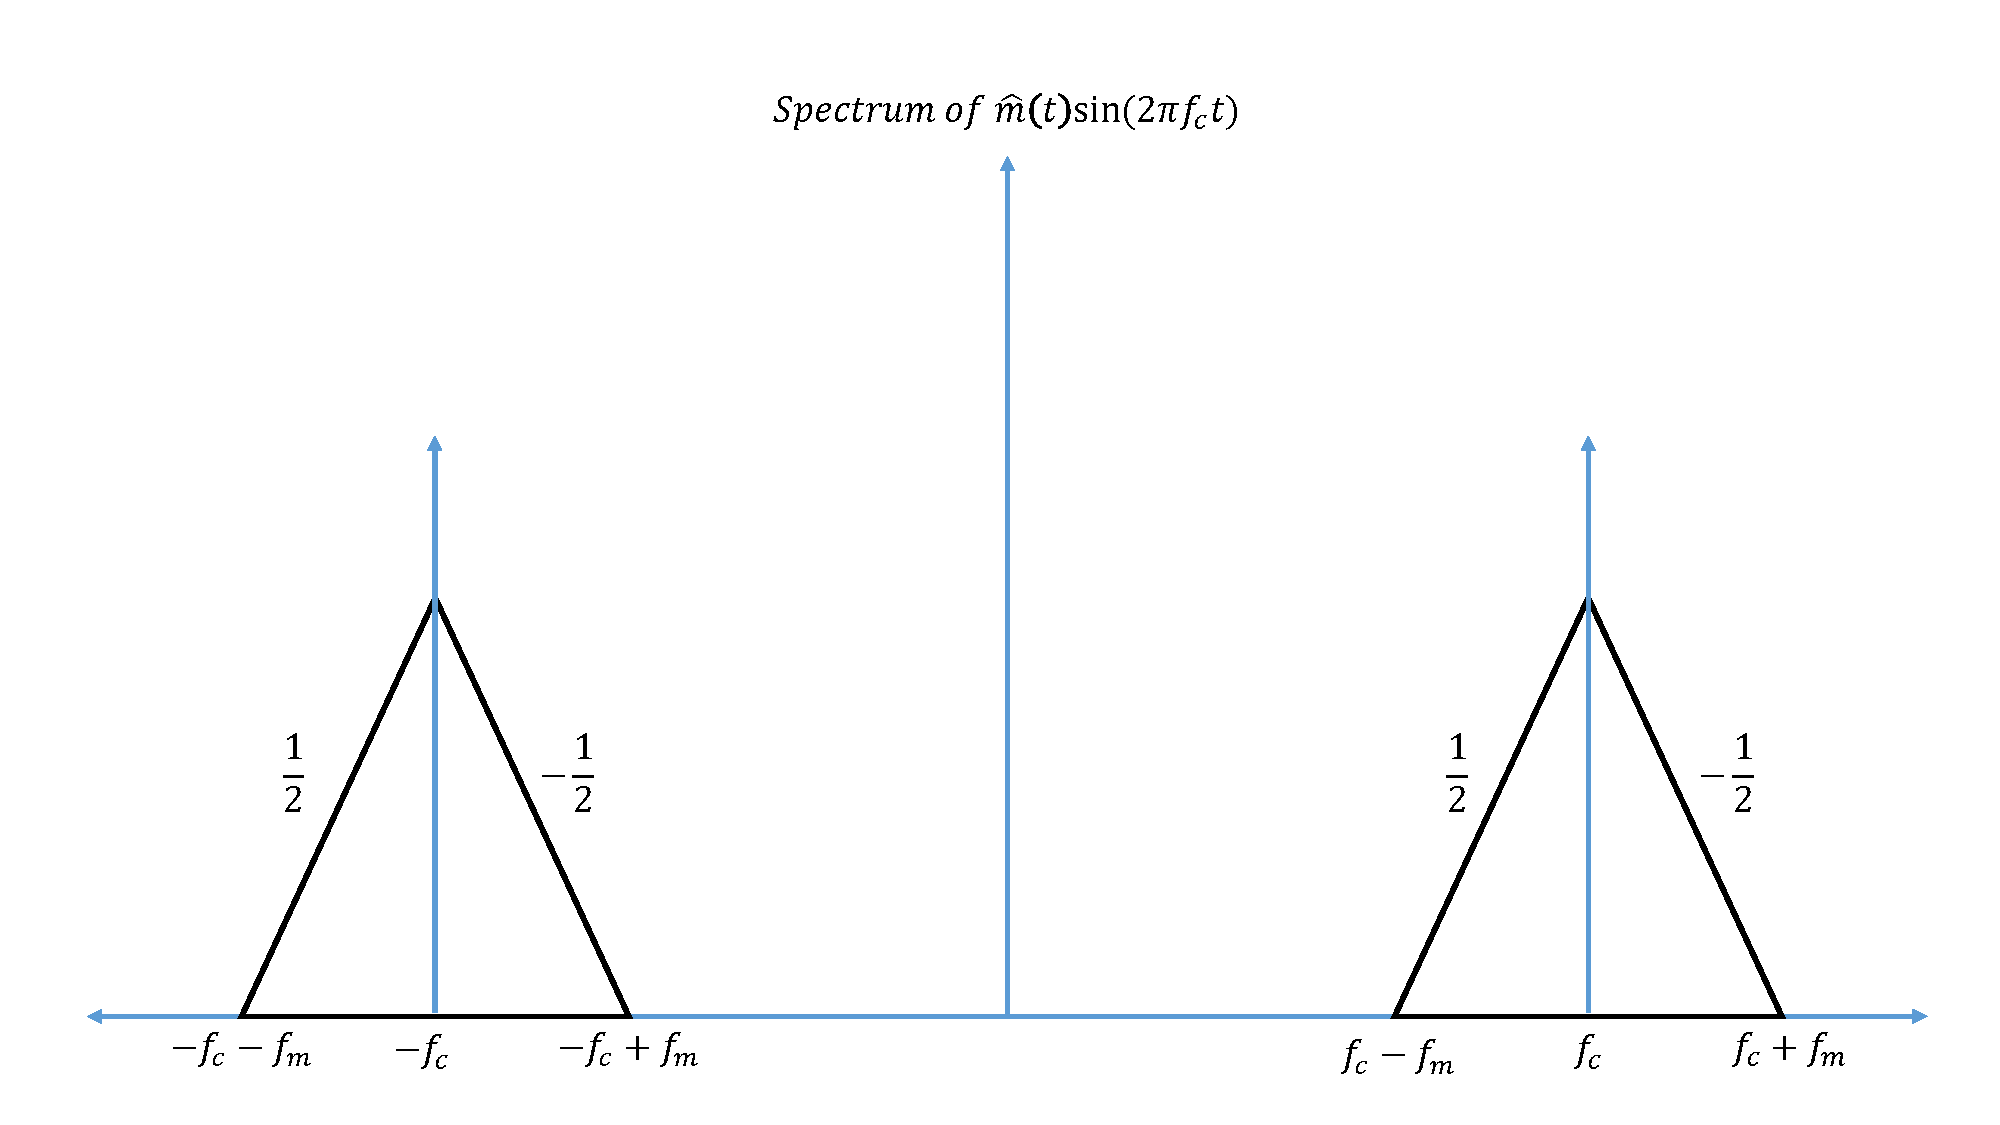
\includegraphics[width=1.0\textwidth, height=8cm]{./sdf/simplified_coherent_receiver/figures/SSB5.pdf}
	\caption{Hilbert transformed modulated signal}\label{Hilbert_Final}
\end{figure}

Further, summation of the two signals ${m(t)} cos(2\pi f_c t)$ and ${\hat{m}(t)} sin(2\pi f_c t)$ will generate the upper sideband SSB signal as follows,
\begin{equation}
u(t)={m(t)} cos(2\pi f_c t)-{\hat{m}(t)} sin(2\pi f_c t)
\label{5.23}
\end{equation}
From the above discussion, the spectrum of the Equation \ref{5.23} can be given by the Figure \ref{SSB_signal_spectrum}. Similarly, for the lower sideband SSB can be generated by Equation,
\begin{equation}
u(t)={m(t)} cos(2\pi f_c t)+{\hat{m}(t)} sin(2\pi f_c t)
\label{5.24}
\end{equation}
\begin{figure}[h]
	\centering
	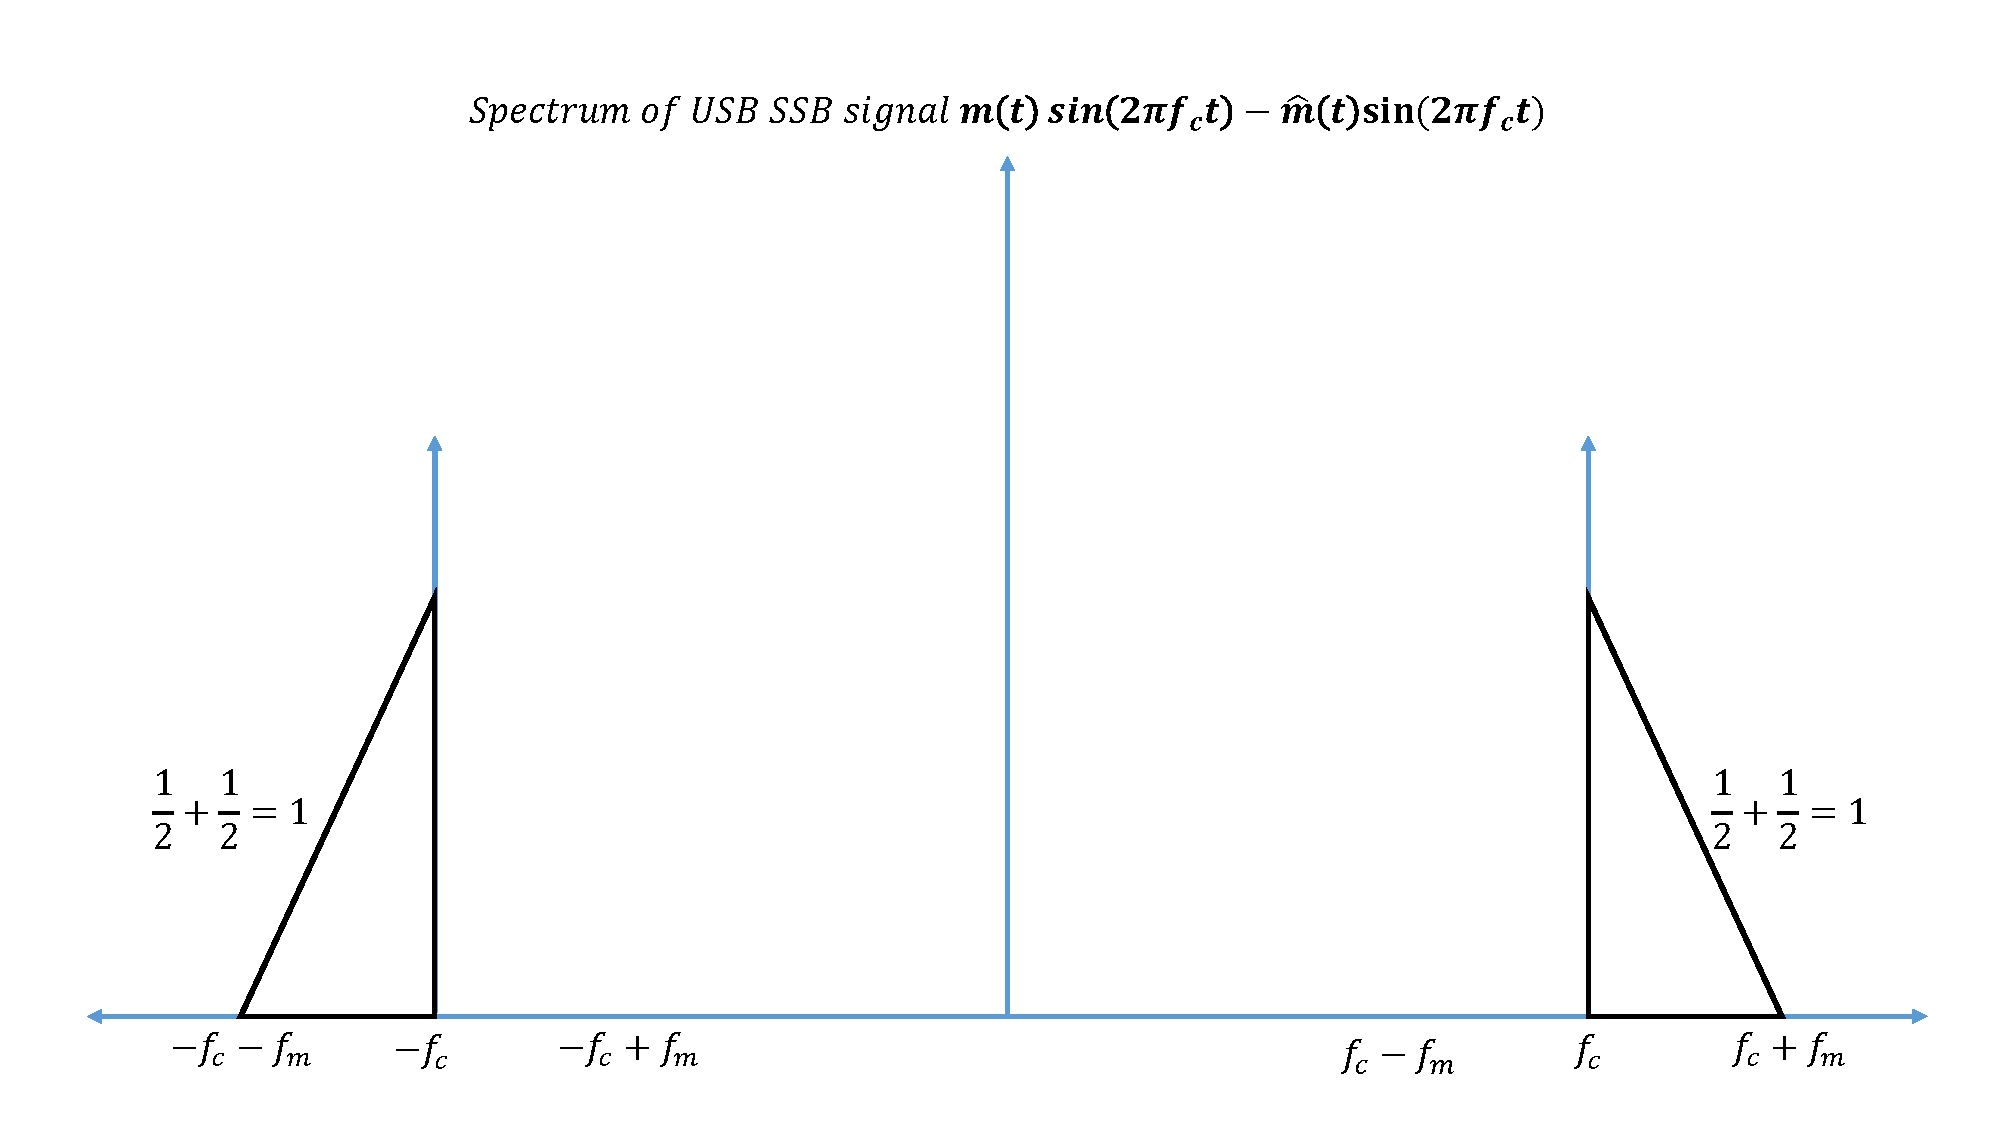
\includegraphics[width=1.0\textwidth, height=8cm]{./sdf/simplified_coherent_receiver/figures/SSB6.pdf}
	\caption{SSB signal spectrum}\label{SSB_signal_spectrum}
\end{figure}

\subsubsection{Kramers Kronig Relation}
Suppose we have a SSB signal $u(t)$ described as,
\begin{equation}
u(t)=u_r(t)+iu_i(t)
\label{Eq:5.22}
\end{equation}
In the equation \ref{Eq:5.22}, the real and imaginary parts $U_r(t)$ and $U_i(t)$ are related through the Kramers-Kronig relation with each other. An intuitive way to analyze the relation is based on expressing its Fourier transform $\tilde{U}(\omega)$ as follows,
\begin{equation}
\tilde{U}(\omega)=\dfrac{1}{2}[1+sgn(\omega)]\tilde{U}(\omega)
\label{Eq:5.23}
\end{equation}
The equation \ref{Eq:5.23} follows the SSB signal condition $\tilde{U}(\omega)=0$ for $\omega<0$. Further, simplification0n of the signal can be summarized as follows:
\begin{equation}
\begin{split}
\tilde{U}(\omega)&=\dfrac{1}{2}[1+sgn(\omega)]\tilde{U}(\omega)\\
				 &=\dfrac{1}{2}\tilde{U}(\omega)+\dfrac{1}{2}sgn(\omega)\tilde{U}(\omega)
\end{split}
\label{Eq:5.23}
\end{equation}
Taking inverse Fourier transform of the equation \ref{Eq:5.23},
\begin{equation}
\begin{split}
	{u}(t)&=IFT\{\tilde{}(\omega)\}\\
	      &=\dfrac{1}{2}{u}(t)+\underline{\dfrac{1}{2}[IFT\{sgn(\omega)\} \circledast {u}(t)]}
\end{split}
\label{Eq:5.23}
\end{equation}
The underlined term in Equation \ref{Eq:5.23} displays that multiplication in frequency domain converted into the convolution in the time domain. Further, IFT of the function $sgn(\omega)$ given as $(-i/\pi t)$. As a consequences, we can further simplify our equation as,
\begin{equation}
\begin{split}
{u}(t)&=\dfrac{1}{2}{U}(t)+\frac{1}{2}\bigg[\frac{i}{\pi t} \circledast {u}(t) \bigg]\\
\frac{{u}(t)}{2} &=\frac{1}{2}\bigg[\frac{i}{\pi t} \circledast {u}(t) \bigg]\\
{u}(t) &=i\bigg[\frac{1}{\pi t} \circledast {u}(t) \bigg]\\
{u}(t) &=\frac{i}{\pi} p.v. \int_{-\infty}^{\infty} \frac{u(t')}{t-t'} dt' 
\end{split}
\label{Eq:5.24}
\end{equation}
Using Equation \ref{Eq:5.23} into Equation \ref{Eq:5.24},
\begin{equation}
\begin{split}
u_r(t)+iu_i(t) &=\frac{i}{\pi} p.v. \int_{-\infty}^{\infty} \frac{u(t')}{t-t'} dt' 
\end{split}
\label{Eq:5.24}
\end{equation}
Therefore,
\begin{equation}
\begin{split}
u_r(t)+iu_i(t) &=\frac{i}{\pi} p.v. \int_{-\infty}^{\infty} \frac{u_r(t')+iu_i(t')}{t-t'} dt' \\
u_r(t)+iu_i(t)&=-\frac{1}{\pi} p.v. \int_{-\infty}^{\infty} \frac{u_i(t')}{t-t'} dt' + \frac{i}{\pi} p.v. \int_{-\infty}^{\infty} \frac{u_r(t')}{t-t'} dt'
\end{split}
\label{Eq:5.24}
\end{equation}
which leads to,
\begin{equation}
\begin{split}
u_r(t) &=-\frac{1}{\pi} p.v. \int_{-\infty}^{\infty} \frac{u_i(t')}{t-t'} dt' \\
u_i(t) &=\frac{1}{\pi} p.v. \int_{-\infty}^{\infty} \frac{u_r(t')}{t-t'} dt' \\
\end{split}
\label{Eq:5.24}
\end{equation}





  



\subsection{Rx side}
At the receiver side, signal is coherently detected using a simplified coherent receiver and a local oscillator. The optical signal is then converted into the electrical domain using two balanced photodetector (BPD), or alternatively four photodetector, and amplified by a transimpedance amplifier (TIA). Following that, the signals are sampled by two 8-bit 2.5 GSa/s ADC and the this digitized signal sent to the FPGA (Virtex-7) where all post-detection DSP implemented in real-time.

\begin{thebibliography}{9}
	\bibitem{latexcompanion}
	Antonio Mecozzi, Cristian Antonelli, and Mark Shtaif.
	\textit{Kramers-Kronig Coherent Receiver}.
	Optica, vol.3, no.11, 2016, p.1220., doi:10.1364/optica.3.001220.
	
	\bibitem{latexcompanion}
	Antonio Mecozzi.
	\textit{Retrieving the full optical response from amplitude data by Hilbert transform}. Opt. Comm. 282, 4183-4187.
	
	\bibitem{latexcompanion}
	Antonio Mecozzi.
	\textit{A necessary and sufficient condition for minimum phase and implication of phase retrieval}. arXiv:1606.04861.
\end{thebibliography}


